\documentclass[11pt,a4paper]{article}
% Windows
%\usepackage[cp1250]{inputenc}
%\usepackage[polish]{babel}

% Linux
\usepackage{polski}
\usepackage[utf8]{inputenc}

% Dodatkowe paczki
\usepackage{graphicx} % \includegraphics OBRAZ
\author{Łukasz Radzio}
\title{Sprawozdanie 1.\\ Optymalizacja w kierunku }
% \\ nowa linia
\date{Wtorek 8.00\\8.03.2016}


\begin{document}
\maketitle
%\section{Wstêp}
\section*{PODSTAWY}
\subsection*{RÓWNANIA}% gwiazdka bez numeru
Znaleźć wszystkie rzeczywiste pierwiastki wielomianu:
\[w(x)=x^3-91.11x^4-899.989x^3+1100.009x^2-11.091x+1\]
Poprzez minimalizację
\newline % bez wcięcia
\\ %newline
I am higher than everyone.

Z wcięciem $ E=mc^2 $ w tekście.
$$ E = mc^2 $$ % również nienumerowane
\begin{equation} % numerowane
	E=mc^2 + 1
\end{equation}

\subsection*{KOD}
\begin{verbatim} 
clear all
tic
global a %zmienna globalna wykorzystywana w funkcji koszt
a = [1 -91.11 -899.989 1100.009 -110.91 1]; %wsp. 
\end{verbatim}

\subsection*{WYLICZENIA}
\texttt{prosta1} \textbf{pr}osta1:
\begin{enumerate}
	\item $x_{0}=0$ - punkt startowy.
	\item $d=0.01$ - kierunek..
\end{enumerate}
\begin{itemize}
	\item $x_{0}=0$ - punkt startowy.
	\item $d=0.01$ - kierunek..
\end{itemize}
\newpage
\section*{TABELA}
\begin{table}[h]
	\centering
	\caption{Porównanie wyników}
	\begin{tabular}{|c|c|c|}
		\hline
		Rozwiązanie rzeczywiste & Rozwiązanie numeryczne  & Różnica\\
		\hline
		0.01    &  0.01  & 0\\
		\hline
		0.1  &  0.100000000274571  & $2.70\cdot10^{-10}$\\
		\hline
		1  &  0.999999998950029  & $1.05\cdot10^{-9} $\\
		\hline
		-10  &  -9.999999989840209  & $1.02\cdot10^{-8} $\\
		\hline
		100  &  99.999999990615620  & $9.38\cdot10^{-9} $\\
		\hline		
		\end{tabular}
\end{table}

\section*{OBRAZ}
\begin{figure}[h]
	\centering
	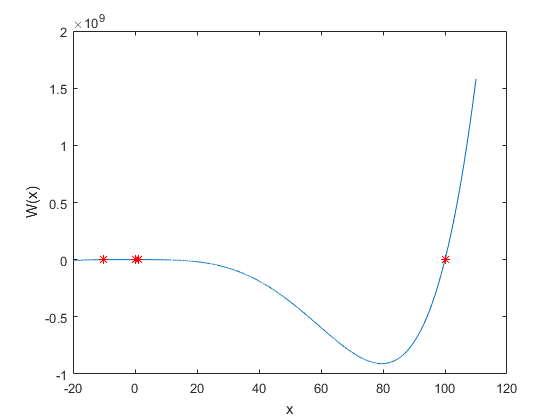
\includegraphics[width=13cm]{obrazDo_Szablonu.png}
	\caption{Wykres funkcji: $w(x)=x^3-91.11x^4-899.989x^3+1100.009x^2-11.091x+1$. Z zaznaczonymi na czerwono wyliczonymi  miejscami zerowymi}
\end{figure}

\end{document}